\documentclass{article}

\usepackage{graphicx}
\usepackage{listings}

\graphicspath{ {./images/} }

\title{Matlabintro}
\author{Pølse}

\lstset{literate={á}{{\'a}}1 {é}{{\'e}}1 {í}{{\'i}}1 {ó}{{\'o}}1 {ú}{{\'u}}1 {Á}{{\'A}}1 {É}{{\'E}}1 {Í}{{\'I}}1 {Ó}{{\'O}}1 {Ú}{{\'U}}1 {à}{{\`a}}1 {è}{{\`e}}1 {ì}{{\`i}}1 {ò}{{\`o}}1 {ù}{{\`u}}1 {À}{{\`A}}1 {È}{{\'E}}1 {Ì}{{\`I}}1 {Ò}{{\`O}}1 {Ù}{{\`U}}1 {ä}{{\"a}}1 {ë}{{\"e}}1 {ï}{{\"i}}1 {ö}{{\"o}}1 {ü}{{\"u}}1 {Ä}{{\"A}}1 {Ë}{{\"E}}1 {Ï}{{\"I}}1 {Ö}{{\"O}}1 {Ü}{{\"U}}1 {â}{{\^a}}1 {ê}{{\^e}}1 {î}{{\^i}}1 {ô}{{\^o}}1 {û}{{\^u}}1 {Â}{{\^A}}1 {Ê}{{\^E}}1 {Î}{{\^I}}1 {Ô}{{\^O}}1 {Û}{{\^U}}1 {œ}{{\oe}}1 {Œ}{{\OE}}1 {æ}{{\ae}}1 {Æ}{{\AE}}1 {ß}{{\ss}}1 {ç}{{\c c}}1 {Ç}{{\c C}}1 {ø}{{\o}}1 {å}{{\r a}}1 {Å}{{\r A}}1 {€}{{\EUR}}1 {£}{{\pounds}}1
}

\begin{document}
\maketitle
\tableofcontents
\pagebreak

\section{Introduktion till Matlab}
\begin{enumerate}
\item
\begin{math}
A=\pi r^2
\\
r=4
\\
A=\pi*4^2=16\pi=50.2655
\end{math}

\item
\subsection*{}
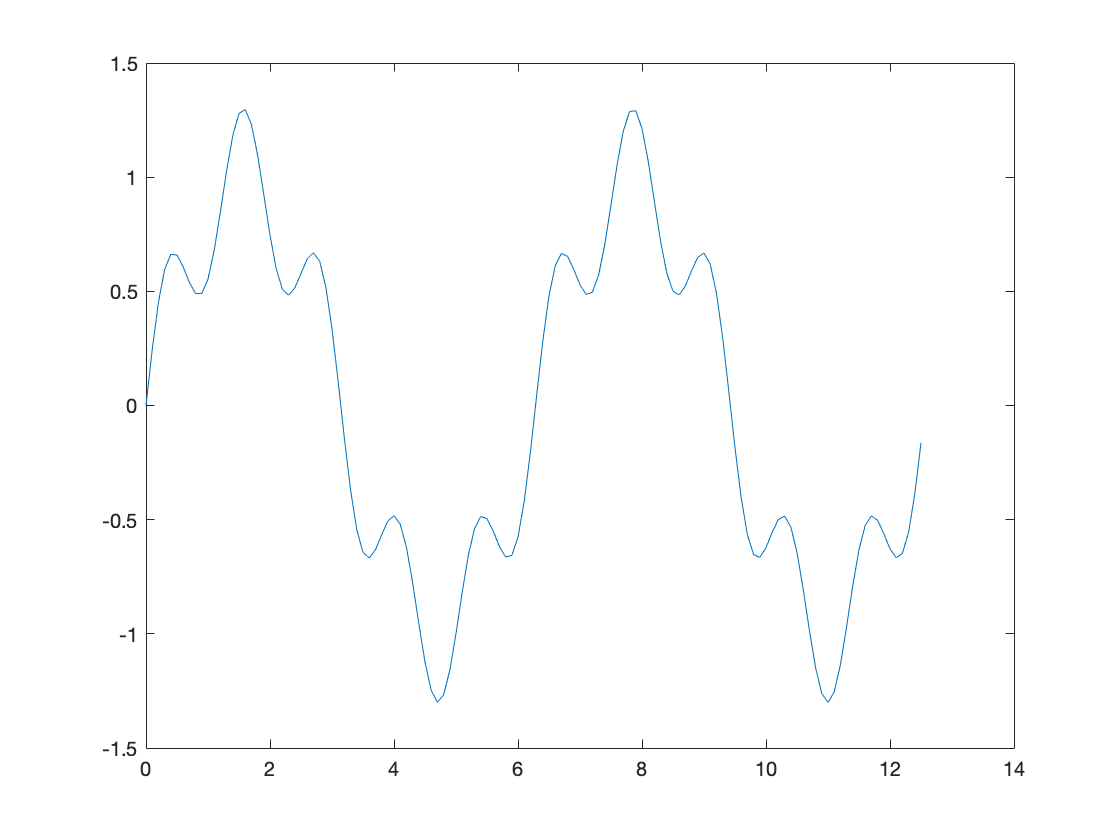
\includegraphics[scale=0.2]{2.png}

\item
\begin{lstlisting}[language=matlab]
s=0;
for i=1:5
    s=s+(i^2);
end
disp("Sum is")
disp(s)
\end{lstlisting}

\item
-0.8241 \& 0.8241

\item
\begin{enumerate}
\item
y = linspace(x1,x2,n) generates n points. The spacing between the points is (x2-x1)/(n-1). \\
y = linspace(x1,x2) returns a row vector of 100 evenly spaced points between x1 and x2.

\item
gg ez

\end{enumerate}

\end{enumerate}

\pagebreak
\section{Kontrollstrukturer och funktioner i Matlab}

\begin{enumerate}

\item
\begin{lstlisting}[language=matlab]
if a<b
    c=a
else
    c=b
end
\end{lstlisting}

\item
\begin{enumerate}
\item
36569 iterations

\item
0.785148163459949

\end{enumerate}

\item
\begin{lstlisting}[language=matlab]
function Omkrets=polylen(x,y)
    n=length(x);
    Omkrets=0;
    for i=1:n-1
        Omkrets=Omkrets+sqrt((x(i+1)-x(i))^2+(y(i+1)-y(i))^2);
    end
\end{lstlisting}

\item
\begin{lstlisting}[language=matlab]
subplot(1,2,1)
axis([-1 1 -2 2])

[x,y]=ginput;
x=[x; x(1)];
y=[y; y(1)];

plot(x,y,"-o")
axis([-1 1 -2 2])

subplot(1,2,2)
fill(x,y,"g")
axis([-1 1 -2 2])
\end{lstlisting}

\end{enumerate}

\pagebreak
\section{Matriser och vektorer i Matlab}

\begin{enumerate}

\item
\begin{lstlisting}[language=matlab]
A=[1 4 7 10; 2 5 8 11; 3 6 9 12];
B=[4 5 6; 3 2 1; 1 1 1];
C=[1; 3; 5];
D=[0 2 4];
\end{lstlisting}

\begin{enumerate}

\item
\begin{lstlisting}[language=matlab]
A=[A(:,1:2) c A(:,3:4)];
B=[B(1,:); d; B(2:3,:)];
\end{lstlisting}

\item
\begin{lstlisting}[language=matlab]
A=[A(3,:); A(2,:); A(1,:)];
A=[A(:,1) A(:,4) A(:,3) A(:,2) A(:,5)];
\end{lstlisting}

\end{enumerate}

\item
\begin{lstlisting}[language=matlab]
b1=[4; 3; 1];
b2=[5; 2; 1];
b3=[6; 1; 1];

B=[b1 b2 b3];
\end{lstlisting}

\item
\begin{lstlisting}[language=matlab]
A=[10 7 8 7; 7 5 6 5; 8 6 10 9; 7 5 9 10];

A11=A([1 2],[1 2]);
A12=A([1 2],[3 4]);
A21=A([3 4],[1 2]);
A22=A([3 4],[3 4]);

A=[A11 A12; A21 A22];
\end{lstlisting}

\item
\begin{lstlisting}[language=matlab]
A=[11 4 3 7; 2 6 8 5; 9 12 1 10];
b=[3; 1; 5];
c=[4 2 8 0 6];

size(b); % 3, 1
size(c); % 1, 5
% b har endast en kolonn -> kolonnvektor
% c har endast en rad -> radvektor

[v,i]=max(A);
[max_el,j_max]=max(v);
i_max=i(j_max);
% största elementet är 12 och finns på (3,2)

[v,i]=min(A);
[min_el,j_min]=min(v);
i_min=i(j_min);
% minsta elementet är 1 och finns på (3,2)
\end{lstlisting}

\item
\begin{lstlisting}[language=matlab]
t=1:5;
v=t .^ 2;
s=sum(v);

v=[1:5] .^ 2;
s=sum(v);

t=1:5;
s=sum(t .^ 2);

s=sum([1:5] .^ 2);
\end{lstlisting}

\item
\begin{lstlisting}[language=matlab]
A=[1 5 9; 2 6 10; 3 7 11; 4 8 12];
B=[4 5 6; 3 2 1; 1 1 1];
x=[1; 1; 1];
a=[-1 0 1];

Ax=A*x; % Ax=[15; 18; 21; 24]
Bx=B*x; % Bx=[15; 6; 3]
AB=A*B; % AB=[28 24 20; 36 32 28; 44 40 36; 52 48 44]
ax=a*x; % ax=[0]
xa=x*a; % xa=[-1 0 1; -1 0 1; -1 0 1]
aB=a*B; % aB=[-3 -4 -5]

[m,n]=size(A);
p=size(x,2);
C=zeros(m,p);
for i=1:m
    for j=1:p
        cij=0;
        for k=1:n
            cij=cij+A(i,k)*x(k,j);
        end
        C(i,j)=cij;
    end
end
\end{lstlisting}

\item
\begin{lstlisting}[language=matlab]
A=[1 0 0; 0 1 0; 1 0 1];
B=[1 0 0; -2 1 0; 0 0 1];
C=[2 1 1; 4 1 0; -2 2 1];
\end{lstlisting}

\begin{enumerate}

\item
\begin{lstlisting}[language=matlab]
isequal(A*(B*C), (A*B)*C); % -> True
isequal(A*(B+C), A*B+A*C); % -> True
isequal((B+C)*A, B*A+C*A); % -> True    
\end{lstlisting}

\item
\begin{lstlisting}[language=matlab]
isequal(A*C, C*A); % -> False
isequal(B*C, C*B); % -> False
isequal(A*B, B*A); % -> True
\end{lstlisting}

\end{enumerate}

\end{enumerate}

\end{document}
